\documentclass[12pt, letterpaper, twoside]{article}
\usepackage{graphicx}
\usepackage[utf8]{inputenc}
\usepackage{longtable}

\title{AI607 Homework 1 Report}
\author{20214487 Geonju Lee}

\begin{document}

\maketitle

\section{In-degree and Out-degree}

\begin{center}
% \begin{tabular*}{\textwidth}{ c c }
\begin{longtable}{ c c }  
    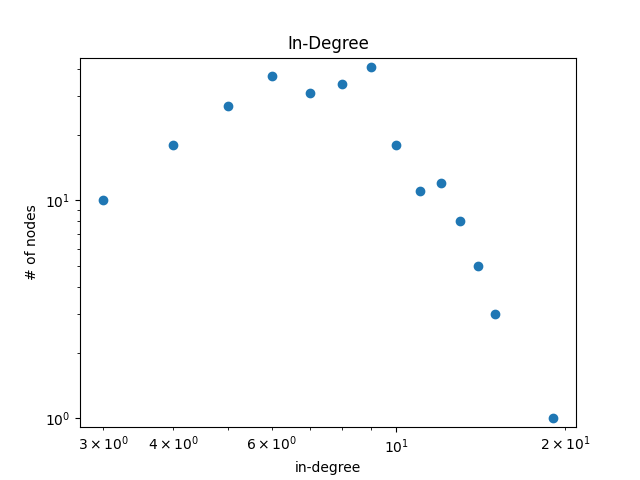
\includegraphics[width=0.5\textwidth]{1S_indeg.png} 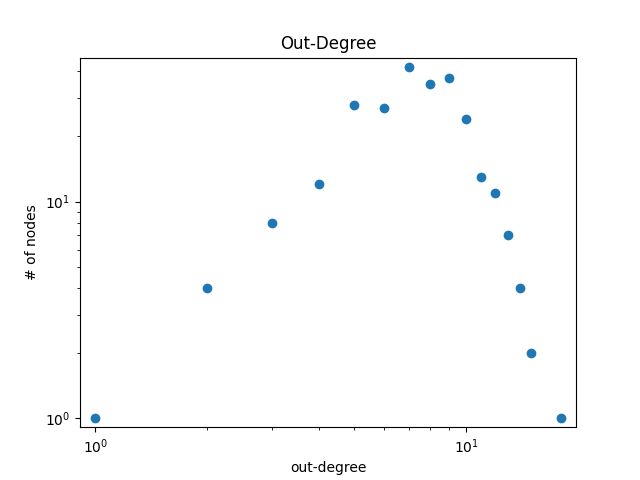
\includegraphics[width=0.5\textwidth]{1S_outdeg.png} \\
    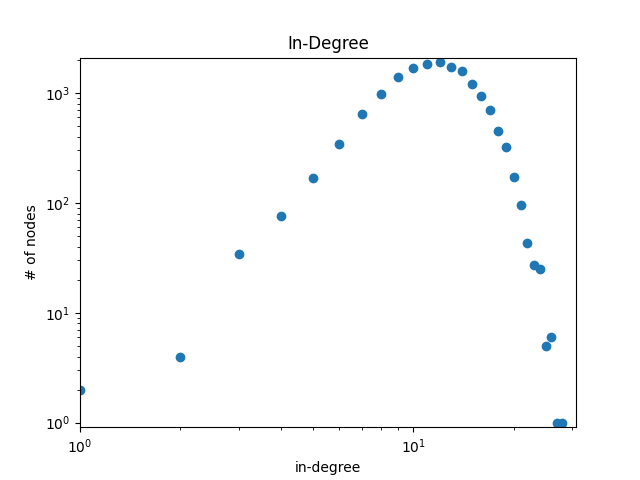
\includegraphics[width=0.5\textwidth]{1L_indeg.png} 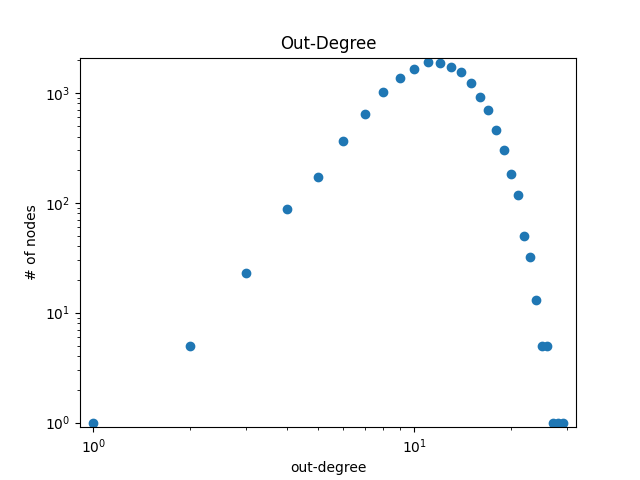
\includegraphics[width=0.5\textwidth]{1L_outdeg.png} \\
    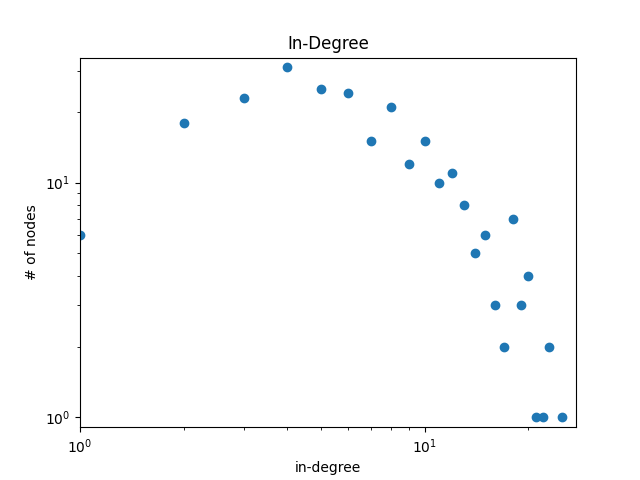
\includegraphics[width=0.5\textwidth]{2S_indeg.png} 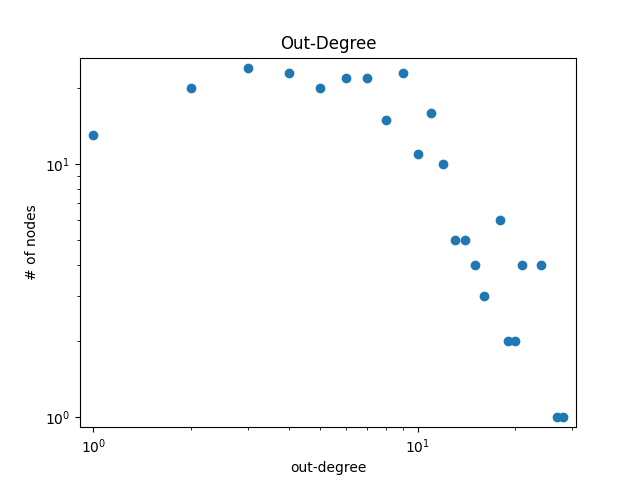
\includegraphics[width=0.5\textwidth]{2S_outdeg.png} \\
    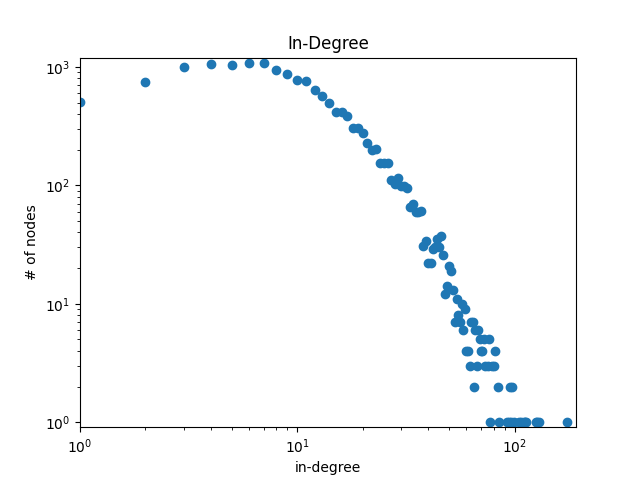
\includegraphics[width=0.5\textwidth]{2L_indeg.png} 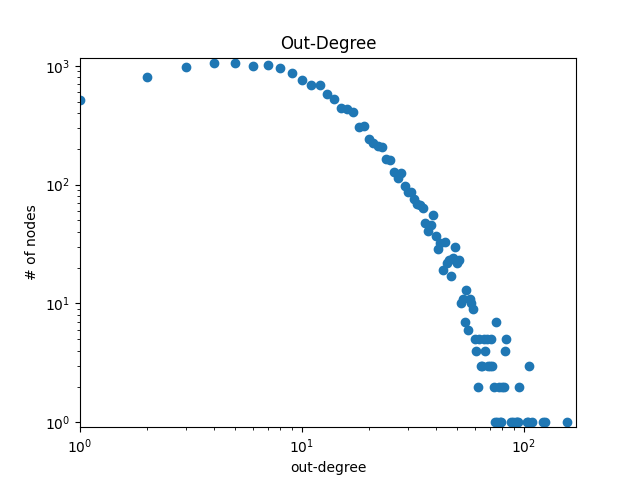
\includegraphics[width=0.5\textwidth]{2L_outdeg.png} \\
    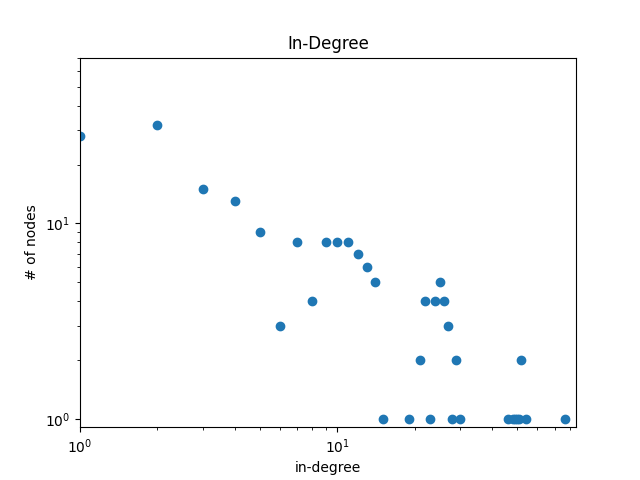
\includegraphics[width=0.5\textwidth]{3S_indeg.png} 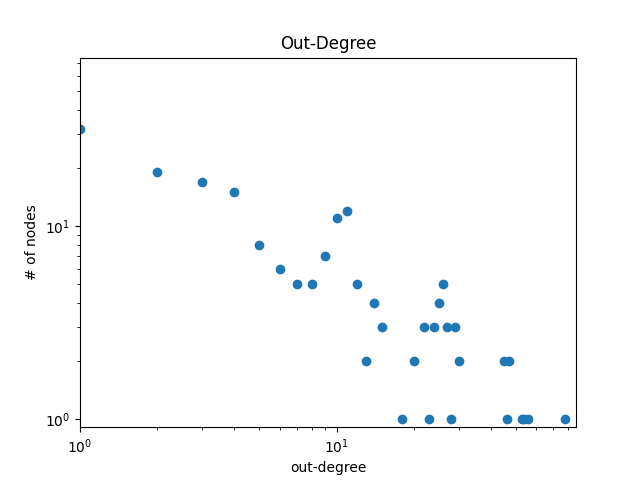
\includegraphics[width=0.5\textwidth]{3S_outdeg.png} \\
    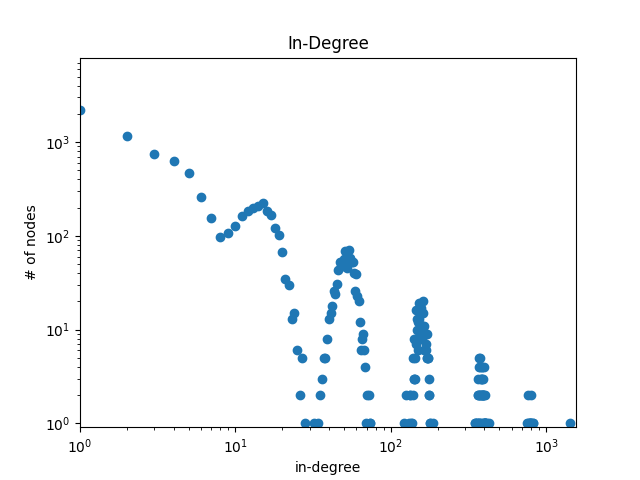
\includegraphics[width=0.5\textwidth]{3L_indeg.png} 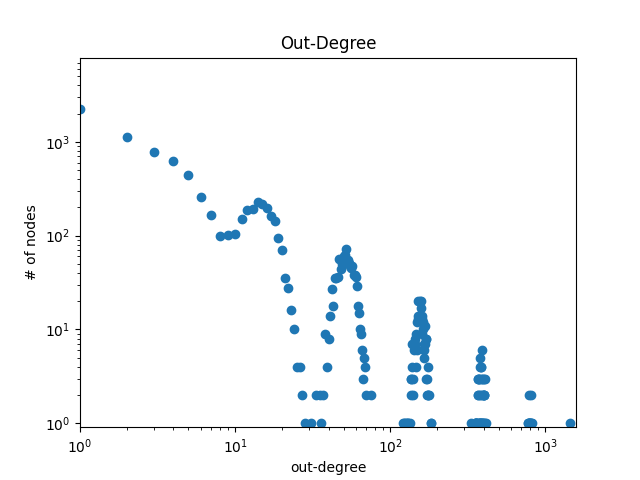
\includegraphics[width=0.5\textwidth]{3L_outdeg.png} \\
\caption{Plots of the in- and out- degree distributions of $G_{1,S}$, $G_{1,L}$, $G_{2,S}$, $G_{2,L}$, $G_{3,S}$ and $G_{3,L}$ from top to bottom; in-degree plots on the left side and out-degree plots on the right side.}
\end{longtable}
% \end{tabular*}

\end{center}

\section{Singular values}

\begin{center}
    % \begin{tabular*}{\textwidth}{ c c }
    \begin{longtable}{ c c }  
        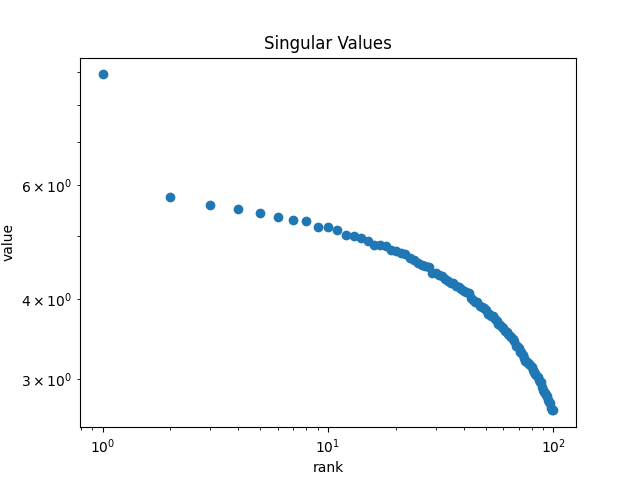
\includegraphics[width=0.5\textwidth]{1S_svd.png} 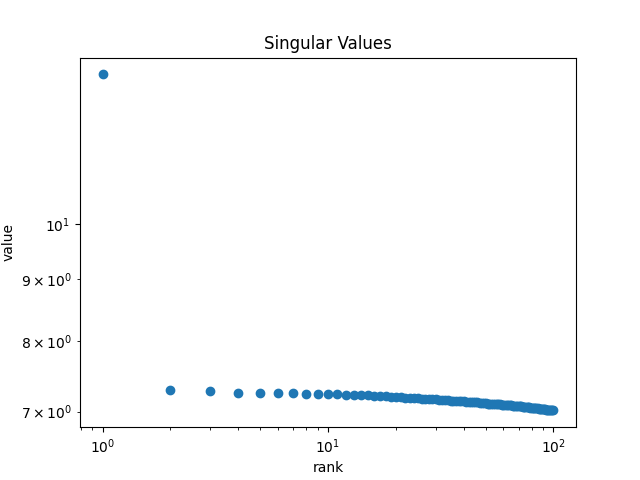
\includegraphics[width=0.5\textwidth]{1L_svd.png} \\
        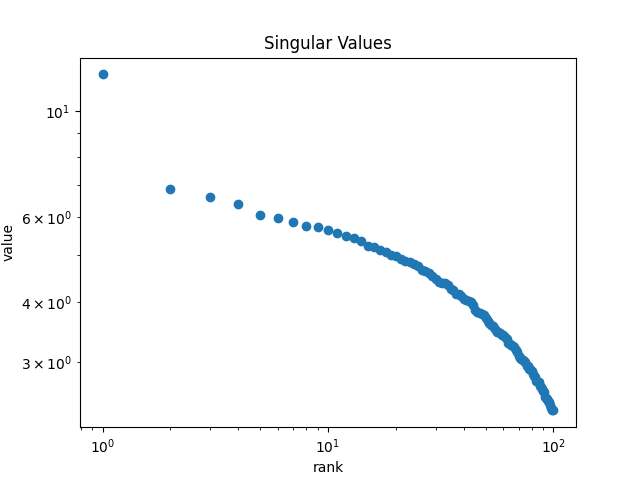
\includegraphics[width=0.5\textwidth]{2S_svd.png} 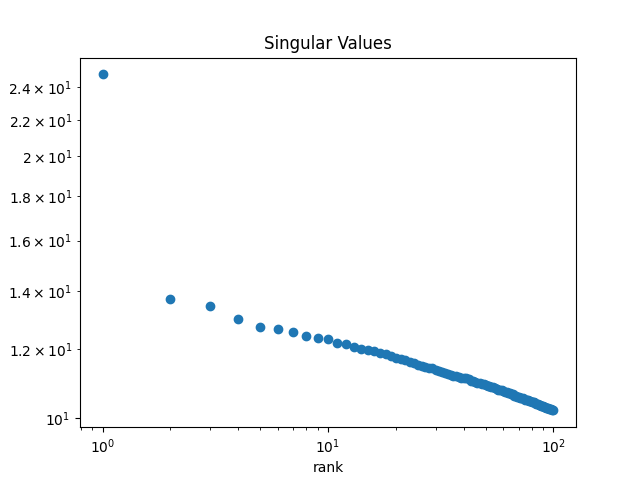
\includegraphics[width=0.5\textwidth]{2L_svd.png} \\
        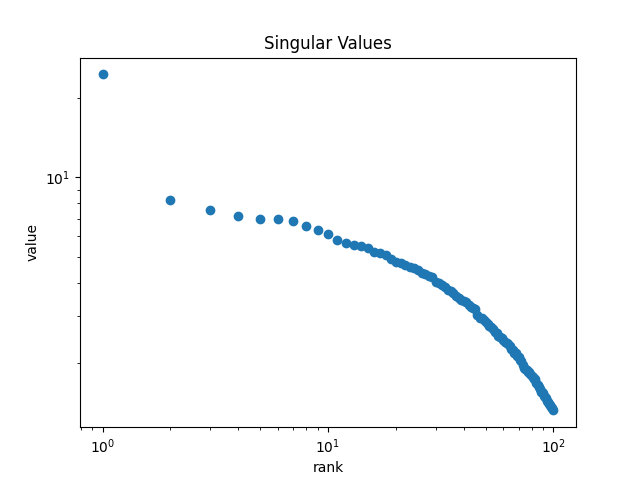
\includegraphics[width=0.5\textwidth]{3S_svd.png} 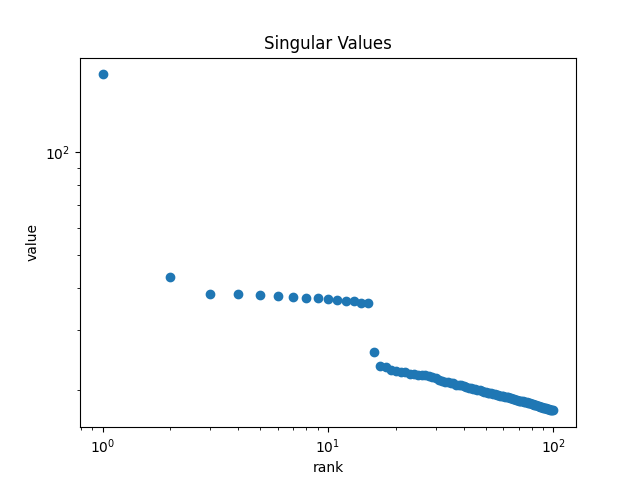
\includegraphics[width=0.5\textwidth]{3L_svd.png} \\
    \caption{Plots of the singular values of $G_{1,S}$, $G_{1,L}$, $G_{2,S}$, $G_{2,L}$, $G_{3,S}$ and $G_{3,L}$ from left to right, and from top to bottom}
    \end{longtable}
    % \end{tabular*}
    
    \end{center}

\section{Analysis}

The degree distribution follows binomial distribution for S1 and S2, but not for S3; $G_{3,S}$ and $G_{3,L}$ have degree distribution similar to wave form. % power law degree distribution?
In S1 and S2, the probabilities $p_a,p_b,p_c,p_d$ are equal or similar, while they are unequally distributed in S3.

\end{document}